\documentclass[tikz, border = 10pt]{standalone}
\renewcommand{\familydefault}{\sfdefault}

\usetikzlibrary{positioning, calc, quotes, arrows.meta, shapes}

\tikzset{
  every edge quotes/.style = {fill = white},
  > = {Stealth[length = 1.5mm]},
  shorten > = 1pt, 
  shorten < = 1pt, 
  manifest/.style = {draw, inner sep = 3pt, align = center, 
    minimum width = 1cm, minimum height = 0.85cm},
  latent/.style = {manifest, ellipse},
  regression/.style = {->, shorten < = 0pt, inner sep = 1.5pt},
  covariance/.style = {<->, inner sep = 1.5pt},
  variance/.style = {<->, inner sep = 0.5pt} 
}

\begin{document}
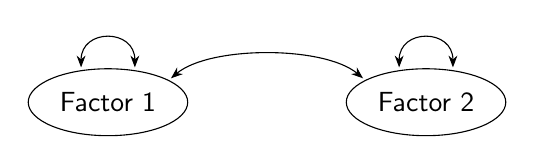
\begin{tikzpicture}

\node [latent] (f1) {Factor 1};
\node [latent] (f2) [right = 2cm of f1] {Factor 2};

\path [covariance] (f1.20) edge [bend left = 40, looseness = 0.7] (f2.160);

\path [variance] (f1.50) edge [bend right = 90, looseness = 2.0] (f1.130);
\path [variance] (f2.50) edge [bend right = 90, looseness = 2.0] (f2.130);

\end{tikzpicture}
\end{document}
